\chapter{Topologie}
Schématiquement, un réseau de communication est composé de terminaux, de noeuds et de liens. Le terme de noeud a été aussi désigné par le nom d'IMP (Interface Message Processor). L'IMP était le n\oe{}ud de commutation de paquets utilisé pour connecter les ordinateurs à l'ARPANET à la fin des années 60 et pendant les années 70. C'était la première génération de ce qui s'appelle aujourd'hui routeur.
\begin{figure}[H]
	\centering
	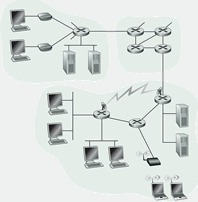
\includegraphics{partie1/reseauschema.jpg}
\end{figure}
\section{Topologie point à point}
L'information est émise d'un terminal à un autre après avoir traversé un ou plusieurs noeuds. Les réseaux à commutation ont cette topologie.
	\subsection{Topologie en étoile}
	Dans la topologie en étoile, le noeud cntral reçoit et envoit tous les messages. L'architcture est simple mais la panne du noeud central paralyse tous les noeuds. D'autre part ce noeud doit avoir les capacités suffisantes pour supporter tout le trafic et le coût en liasions à déployer peut être conséquent
\begin{figure}[H]
	\centering
	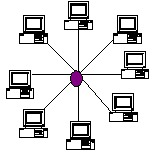
\includegraphics{partie1/topoetoile.jpg}
	\caption{Topologie en étoile}
\end{figure}
	\subsection{Topologie en boucle}
	Dans la topologie en boucle, chaque noeud reçoit un message de son voisin en amont et le retransmet au noeud en aval. Il faut veiller dans certains cas à ce que le noeud émetteur retire le message qui risque de tourner indéfiniment dans le réseau. D'autre part, si un noeud tombe en panne, la boucle est coupée. On peut résoudre cela par une double boucle avec reconfiguration en cas de panne.
\begin{figure}[H]
	\centering
	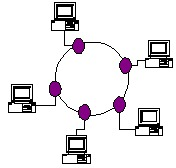
\includegraphics{partie1/topoboucle.jpg}
	\caption{Topologie en boucle}
\end{figure}
	\subsection{Topologie maillée}
	Dans la topologie maillée, on peut avoir une interconnexion complète (maillage régulier) mais cela peut coûter cher en câblage. C'est pourquoi, une étude du trafic permet d'établir une infrastructure de maillage irrégulière. Dans ce cas, il faut prévoir au moins deux routes pour aller d'un point à un autre et un algorithme de routage efficient qui diminue le temps de traversée du réseau. 
\begin{figure}[H]
	\centering
	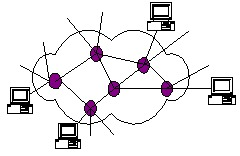
\includegraphics{partie1/topomaille.jpg}
	\caption{Topologie maillée}
\end{figure}
\section{Topologie à diffusion}
\'Egalement appelé broadcast, l'information émise d'un terminal peut être reçue par différents terminaux et même tous les terminaux (message diffusé). Cette possibilité est due au fait que les différents terminaux se partagent un même support. Un des problèmes majeurs dans cette topologie est l'accès au média. Comment peut s'effectuer le contrôle et comment gérer les collisions ? Dans ce paragraphe, nous nous intéressons aux différentes topologies indépendemment de la méthode de partage du support.


\begin{figure}[H]
	\centering
	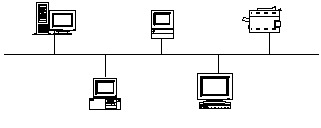
\includegraphics{partie1/topobus.jpg}
	\caption{Topologie en bus}
\end{figure}


\begin{figure}[H]
	\centering
	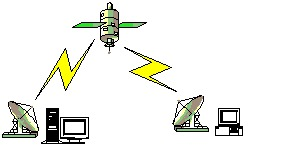
\includegraphics{partie1/toposat.jpg}
	\caption{Topologie Satellite}
\end{figure}

\begin{figure}[H]
	\centering
	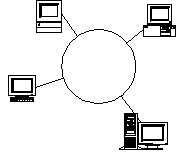
\includegraphics{partie1/toporing.jpg}
	\caption{Topologie en anneau}
\end{figure}

\begin{figure}[H]
	\centering
	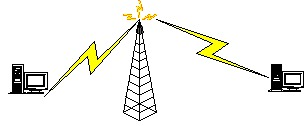
\includegraphics{partie1/toporadio.jpg}
	\caption{Topologie radio}
\end{figure}
Les topologies en bus et en anneau sont essentiellement utilisées dans les réseaux locaux. Dans ces configurations, si le support est coupé, alors le réseau s'arrête. C'est pourquoi, tout en utilisant le mode de diffusion bus ou anneau, l'architecture physique est une architecture en étoile (utilisation de Hub).

\section{Choix d'une topologie}
Toute topologie adoptée doit faire au préalable l'objet d'une étude prenant en compte plusieurs facteurs:

\begin{itemize}
	\item nombre de stations à connecter;
	\item flux des données;
	\item coût;
	\item distance entre entités communicantes;
	\item évolution possible;
	\item résistance aux pannes et lignes de secours;
	\item administration;
	\item \ldots
\end{itemize}

